%% PNAStwoS.tex
%% Sample file to use for PNAS articles prepared in LaTeX
%% For two column PNAS articles
%% Version1: Apr 15, 2008
%% Version2: Oct 04, 2013

%% BASIC CLASS FILE
\documentclass{pnastwo}

%% ADDITIONAL OPTIONAL STYLE FILES Font specification

%\usepackage{pnastwoF}



%% OPTIONAL MACRO DEFINITIONS
\def\s{\sigma}
%%%%%%%%%%%%
%% For PNAS Only:
\url{}
\copyrightyear{}
\issuedate{Issue Date}
\volume{Volume}
\issuenumber{Issue Number}
%\setcounter{page}{} %Set page number here if desired
%%%%%%%%%%%%

\begin{document}

\title{Conflict and Strategy in Collective Computation}

\author{Eleanor Brush\affil{1}{Princeton University, Princeton, NJ, USA}\affil{2}{Wisconsin Institute for Discovery, University of Wisconsin, Madison, USA},
David Krakauer \affil{2}{}\affil{3}{Santa Fe Institute, Santa Fe, USA},
\and
Jessica Flack\affil{2}{}\affil{3}{}}

\contributor{Submitted to Proceedings of the National Academy of Sciences
of the United States of America}

%%%Newly updated.
%%% If significance statement need, then can use the below command otherwise just delete it.
\significancetext{EB did blah DK did blah JC did blah}


\maketitle

\begin{article}
\begin{abstract}
{Function in biological systems emerges from the behavior of tens (e.g. animal social groups) to millions of components (e.g. neural systems), which use imperfect information and have only partially-aligned interests. Components make behavioral decisions in pair-wise interactions. The combined decisions produce system output. The roles of noise and error in collective computation are poorly understood. The leaky-integrator model (LIM) has been used to study neural pair-wise decision-making. Here we modify LIM to study pair-wise decision-making under conflict and error in animal social systems. We extend LIM to study the collective dynamics generating a group level output. Our model system is a macaque society. The decision at the pair-wise level is whether to emit a subordination signal. The output of the collective computation is the distribution of social power (DSP). We study how properties (waiting time, accuracy) of the decision to signal are influenced by signaling conflicts due to variation in strength of the stimulus input (here, asymmetry in fighting ability), and how these decision-level properties impact output properties. We find conflicts in the decision process strongly affect individuals for whom [the average strength of stimulus input] is large by incentivizing accurate signaling. When pairwise decisions are accurate local properties of the decision network are informative about individual state (here, fighting ability). Global properties become informative as accuracy declines, indicating that collective computation becomes nontrivial under error. DSP shape can be controlled by changing the waiting time to decision. The successful use of the LIM in the neural and social contexts suggests general principles of collective computation due to decision-making tradeoffs common across substrates and scales.
}
\end{abstract}

\keywords{collective computation, noisy learning, leaky integrator, decisions, social network, consensus, power}

\dropcap{I}n many biological systems, functional patterns emerge from the interactions of components making decisions under uncertainty. This includes the decision-making behavior of an animal emerging from the firing decisions of billions of neurons, social structures like the distribution of power arising from the status-signaling decisions in chimpanzee and some macaque social groups, the collective motion of fish schools emerging from the velocity and alignment decisions of individual fish, and the toxins produced by quorum sensing bacteria once the bacteria have aggregated at sufficient density (Table \ref{examples}). In each of these examples the components make decisions based on accumulating information extracted from noisy environments. Their joint behavior produces an aggregate-level pattern with fitness consequences for the components and the collective. This two part process, which has now been described in a number of systems, constitutes a collective computation.

An open question is how components should choose their decision-making strategies when there are conflicts of interest between components, perceptual errors, and noisy inputs, in order to collectively compute outputs with positive payoffs. This requires understanding (1) how the strength of the  conflicts of interest and the importance given to properties of a decision, including waiting time and decision accuracy, determine what strategies should be used, (2) how these decision-making strategies impact the collective computation, and (3) how the decisions of the components combine to produce the computation. 

A variety of models, including the sequential probability ratio test (SPRT) and the leaky-integrator model (LIM), have been developed to study how components choose among alternatives in a noisy environment, for example, the firing decisions of neurons during a motion dot coherence task. Both the SPRT and the LIM track the amount of evidence supporting alternative choices. The LIM has the advantage over the SPRT of allowing for memory loss but application of the LIM to explain, for example, neural firing, has been largely phenomenological. Here we develop a LIM by deriving stochastic differential equations that mechanistically specify how information is accumulated by components and used in decision-making. We then extend the LIM in two ways: we introduce a game-theoretic component and we study a network of pairwise decisions generated by our stochastic model to explore how pairwise interactions combine to produce the output and how the output is influenced by the components' strategies. We use published empirical and computational results from work on collective computation in a well-studied model system to justify the form of our equations. The model system is a captive macaque society (\emph{Macaca nemestrina}, n=48, see Appendix Sec. \ref{empirical}) that is characterized by 
%the \emph{minimum degree of relevant complexity}: 
social learning at the individual level, social structures that arise from nonlinear processes and feedback to influence individual behavior, frequent non-kin interactions and multiplayer conflict interactions 
(Appendix, Sec.\ref{XX})\cite {Flack:2007ir, Flack:2006jh, Flack:2006vi, Flack:2005ih, Flack:2005dg, Thierry:2004tj}. 

\section{Model}
\subsection{Model System}
In our model system, a component is an individual monkey and the decision it makes is whether or not to emit a silent-bared teeth display signaling agreement to another monkey to the subordinate role in their relationship. The decision to signal depends on the perceived magnitude of the asymmetry in their fighting abilities. If the asymmetry is perceived to be large, the cost of subordination is smaller than the cost of continued aggression. Encoded in the directed network of subordination signaling decisions is the output of the collective computation: the distribution of social power (DSP). Social power is operationalized as the degree of agreement in the group that an individual is capable of successfully using force during fights. The DSP is known in this system to affect interaction and conflict management cost with, for example, heavy-tailed distributions making otherwise costly conflict management strategies like policing accessible at least to individuals who sit in the tail. The DSP is obtained by quantifying consensus in the network about a node's capacity to use force successfully. Consensus can be measured using several algorithms that return consensus scores for each individual. These algorithms can be viewed as alternative hypotheses for how power is computed in the system (Sec.\ref{computation}). We study how the strength of the stimulus (asymmetry in fighting ability) and the importance of different properties of the decision to signal (waiting time, accuracy) influence what decision-making strategies the animals should use, and how these decision-level properties impact the shape of the DSP. 


\subsection{Stochastic differential equations}    
We first derive a stochastic model describing decisions made about or between pairs of components. In chemical systems, stochastic differential equations are used to describe the dynamics of the concentrations of various solutes, and these Langevin equations can be derived from a mechanistic description of chemical reactions \cite{Gillespie:1992vn,Gillespie:2000fk}. In the decision-making literature the SDEs used to model noisy decision processes are usually formulated without any mechanistic justification. By following the mathematical derivation of the SDEs in chemical systems given by Gillespie \cite{Gillespie:2000fk},  we can derive the SDEs used in the leaky integrator model. In our model system, each component is a monkey accumulating evidence about its ability relative to another monkey by keeping track of the fights it has won and lost. We could use the same derivation to reach a set of SDEs describing the firing rates of neural populations responding to left and right motion in the visual field, the system to which the LIM has been applied most frequently. For more details about this system, see Appendix Sec. XX. 

In our model system, for each pair of monkeys, each has a decision variable, $X_1$ and $X_2$, indicating the evidence that it has accumulated about its ability relative to the other monkey. In the absence of new information, the decision variables leak back towards $0$ with rate $\ell$.  (A table of all variables used in the text is given in Table \ref{variables}.)  If there is no input, then over a period length $\tau$ each decision variable decreases as $X(t+\tau)=(1-\ell\tau)X(t)$. 

If there is input from the environment, each decision variable incorporates the new evidence.  In our model system,  $X_1$ increases by an amount $b$ when monkey $A$ wins a fight against monkey $B$ and decreases by $b$ when it loses, and conversely for $X_2$.  To calculate the variables at time $t+\tau$, we  count how many times each type of input occurred in the time since $t$ and add the changes resulting from these events to the background leaky estimate (as in \cite{Gillespie:2000fk}):
\begin{align*}
X_1(t+\tau)&=(1-\ell\tau)X_1(t)+b\times\# \text{ of times $A$  wins}[t,t+\tau)\\&-b\times\# \text{ of times $B$ wins }[t,t+\tau)
\\ X_2(t+\tau)&=(1-\ell\tau)X_2(t)-b\times\# \text{ of times $A$ wins }[t,t+\tau)\\&+b\times\# \text{ of times $B$ wins }[t,t+\tau). 
\end{align*}

Our first assumption is that the rates at the inputs (fights) occur is constant over time.  We can thus describe the number of each type of event with a Poisson random variable, $N_\text{A}$ and $N_\text{B}$, giving 
\begin{align*}
X_1(t+\tau)&=(1-\ell\tau)X_1(t)+bN_\text{A}-bN_\text{B}
\\ X_1(t+\tau)&=(1-\ell\tau)X_2(t)-bN_\text{A}+bN_\text{B}.
\end{align*}
If events happen at a rate $r$ and the event is a win for $A$ with probability $c$ and a win for $B$ with probability $1-c$, then the expectation of $N_A$ and $N_B$ in a period of length $\tau$ are, respectively, $\tau r c$ and $\tau r(1-c)$. In our model system, $c$ is related to the strength of the asymmetry in the monkeys' abilities. In the neural case, $c$ is related to the ``coherence'' of the visual stimulus.  A value of $c$ close to $0$ or $1$ means that most of the events are of one type or the other and the decision is easier to make than when $c$ is close to $.5$.

If enough events happen in the period of time from $t$ to $t+\tau$ then we can approximate the Poisson random variables with normal random variables with mean and variance equal to the mean of the Poisson random variables.  Our second assumption, then, is that the period of time of length $\tau$ is long enough to make this approximation. Let $Z_\text{A}$ and $Z_\text{B}$, be independent standard Normal random variables, i.e. with mean $0$ and standard deviation $1$, giving
\begin{align*}
X_1(t+\tau)&=(1-\ell\tau)X_1(t)+b\bigg(\tau rc+\sqrt{\tau rc}Z_{\text{A}}\bigg)\\&-b\bigg(\tau r(1-c)+\sqrt{\tau r(1-c)}Z_{\text{B}}\bigg)
\\X_2(t+\tau)&=(1-\ell\tau)X_2(t)-b\bigg(\tau rc+\sqrt{\tau rc}Z_{\text{A}}\bigg)\\&+b\bigg(\tau r(1-c)+\sqrt{\tau r(1-c)}Z_{\text{B}}\bigg).
\end{align*}
Finally, as we make the period of time shorter and shorter, making $\tau$ infinitesimally small, these equations become stochastic differential equations,
\begin{equation*}
\begin{array}{ll}
dX_1&=\bigg(-\ell X_1(t)+br(2c-1)\bigg)dt+\bigg(b\sqrt{rc}\bigg)dW_\text{A}t\\&-\bigg(b\sqrt{r(1-c)}\bigg)dW_\text{B}t
\\dX_2&=\bigg(-\ell X_2(t)-br(2c-1)\bigg)dt-\bigg(b\sqrt{rc}\bigg)dW_\text{A}t\\&+\bigg(b\sqrt{r(1-c)}\bigg)dW_\text{B}t,
\end{array}
\end{equation*}
where $dW_{\text{A}}$ and $dW_{\text{B}}$ are independent Brownian motions representing, respectively, the wins and losses for monkey $A$.  The assumptions about the timescales on which inputs occur are reasonable in the social system, and the successful application of this type of model to neural populations implies they are not unreasonable in that system.  In Table \ref{variables}, we list the inputs, outputs, and variables of the decision model and how they should be interpreted in the social and neural systems.


\subsection{Reaching a decision}
There are two ways to use the decision variables $X_1$ and $X_2$ to make a decision.  If the difference in the variables can be observed, it indicates the relative strengths of the evidence for each option. If $Y=X_1-X_2$, the system should decides on $X_1$ when $Y$ is large and positive and on $X_2$ when $Y$ is large and negative.  Specifically, there are two thresholds, $T_1$ and $T_2$ such that if $Y>T_1$ the decision is for $X_1$ and if $Y<-T_2$ the decision is for $X_2$.  However, it may be the case that the difference in the variables cannot be observed.  In this case, the decision depends on whether $X_1$ or $X_2$ hits a threshold first.  Again, there are two thresholds, $T_1$ and $T_2$, and if $X_2<-T_2$ the decision is for $X_1$ and if the $X_1<-T_1$ the decision is for $X_2$. 

For neural systems, the two stochastic equations describing the activity of the two neural populations integrating environmental evidence are often reduced to the one-dimensional equation describing the difference in the activity levels \cite{Brown:2005fk,Bogacz:2006uq,Feng:2009kl}. The reduced model is easier to analyze, but it assumes a neural mechanism for calculating the difference in activity rates and there is no empirical basis for this. In social systems like our model system, the one dimensional simplification implies a third party evaluating the difference in the evidence each animal has accumulated rather than allowing for the animals to decide themselves based on their accumulating history.  A decision, i.e. the emission of a signal from one of the two animals, is only reached when one of the two animals' decision variable goes below its threshold. Our social system (and probably the neural system as well) is therefore inherently two-dimensional and so our model is formulated this way.  In Table \ref{differences}, we compare properties of the decision process in both systems.

\subsection{Utility of decision}
The thresholds affect how long the decision takes and the probabilities of either outcome.  A ``good'' decision is one that reaches the correct output quickly, i.e.\ the expected time until a decision is reached (decision time, DT) and the probability that an incorrect decision is made (error rate, ER) are low.  However, it is impossible to minimize both simultaneously as waiting longer and accumulating more evidence makes the decision more accurate.  In the social system, an accurate decision occurs when a weaker animal agrees to be subordinate to a stronger one. We also allow for individuals to have preferences for the decisions independent of correctness.  In the social case, the weaker individual may agree to signal because it has perceived a large asymmetry, but its preference may be to be the dominant individual and not to signal. In the neural case, different neural populations may receive different rewards if the decision reaches different outcomes, regardless of which of the alternatives is correct. Each component involved in the decision prefers a different outcome and wants to maximize the probability that the preferred outcome is reached (probability of decision preference being chosen, $\text{DP}_i$). 
To describe the tradeoffs between error rate, decision time, and preference, we quantify the utility of the decision process by introducing three weights, $w_1$, $w_2$, and $w_3$ such that $w_1+w_2+w_3=1$.  These weights describe how the three quantities are prioritized.  For individual $i$, we define
\begin{equation*}
U_{i}=w_1\text{ER}+w_2\text{DT}+w_3(1-\text{DP}_i).
\end{equation*}
The decision is better if $U_i$ is lower.  In the social system, $w_2$ can be interpreted as the cost of fighting since when $w_2$ is higher, the time spent fighting until a decision is reached is more costly.  In the neural system, $w_2$ depends on whatever costs the brain or the whole animal incurs by waiting for a decision. Given that $\text{DP}_1=1-\text{DP}_2$, it is impossible for them both to maximize $\text{DP}_i$, so the decision preference weight $w_3$ indicates the strength of the conflict of interests between components and how stubborn they are about their preferences. In the social system, $w_3$ captures the benefit from being the dominant animal in a pair and the extent to which the weaker animal perceives the subordination contract to be more costly than continued fighting.  

We show in the Appendix (Sec.\ref{X}) that each of the three decision properties, ER, DT, and DP satisfies a partial differential equation that depends on the SDEs and the parameters of the model. There are analytical solutions to these equations when the system of SDEs is reduced to one dimension. However, we were not able to find an analytical solution for the full two-dimensional system and we therefore used numerical methods to solve the PDEs in this case.

\subsection{Nash equilibrium thresholds}
In a group of individuals, each with a value $a_i$, the difficulty with which the pair $i,j$ makes a decision increases with the difference in value, i.e. $c_{ij}$ is an increasing function of $|a_i-a_j|$. In the social system, the value $a_i$ reflects an animal's fighting ability. In the neural system, the value $a_i$ is high if the property (e.g.\ left movement or red color) a neural population responds to is abundant in the visual stimulus. We assume each individual has the same decision threshold for all the decisions processes with each of its peers and, given those thresholds, each individual $i$ has a utility $U_{ij}$ from its decision process with individual $j$ and a total utility given by the average of these, $\langle U_{ij}\rangle _j$. For each set of values $\{a_1,\dots,a_N\}$, we find the Nash equilibrium thresholds such that no individual has an incentive to choose another threshold to improve its utility.  Since the Nash thresholds depend on the values $\{a_1,\dots,a_N\}$,  we repeatedly draw a set of values from a uniform distribution and find the Nash thresholds for each set. Then, for each possible rank $i=1,\dots,N$, we find the average Nash threshold for an individual with the $i^{\text{th}}$ highest ability across these draws.   

\subsection{Collective computation}
\label{computation}
In both the neural system and the social system, the decision can also be thought of as opinions. In the neural system, a decider neuron fires or not in response to some input by upstream neurons, which can be viewed the opinion of the decider node that the relative `value' of one upstream neurons is higher than another. In our model system, the opinion of the sender is that the receiver is capable of using force. In each case, the opinions  in favor of one of each pair of components form a directed network and the collective opinion or degree of consensus in the group about the value of a given component is encoded in this network. In the social case, the degree of consensus about the ability to use force successfully gives a monkey's social power and the distribution of these consensus scores across the group is the distribution of power (Sec. refX) \cite{Brush:2013fk, Flack:2006uq}.

The integration of the opinions about or between each pair of components into a set of consensus scores is the collective computation. There are a number of algorithms that can be used to compute how much consensus there is in a network about the value of each component \cite{Brush:2013fk, Flack:2006uq}.  Here we ask which consensus algorithm is most informative about the components' values and would therefore be the best with which to perform the collective computation. To do this, we use the algorithms to compute a DSP from networks generated by our stochastic model of decision-making and ask which model-generated DSP is most informative about the underlying fighting abilities in the model. 

The simplest algorithm is the unweighted in-degree of a node, i.e. the number of opinions in favor of each individual.  The second algorithm we consider is the weighted in-degree of a node, which is a finer measure than the unweighted in-degree since it takes into consideration the strength of each opinion in favor of the node.  The third is the entropy of the distribution of the number of opinions in favor of each individual, which gives a coarse measurement of how uniformly all other individuals in the group behave with respect to a focal individual.  The fourth is the eigenvector centrality of the network, which measures how central each node is in the global structure of the network.  For more details see \cite{Brush:2013fk}. Using many random sets of values $\{a_1,\dots,a_n\}$ to generate thresholds $\{T_1,\dots,T_N\}$ and then a directed network, we find the mutual information between the consensus scores from the networks and the values, for each consensus algorithm. We also find the average skewness of the set of consensus scores given by each algorithm.

To create a directed network, for each set of values $\{a_1,\dots,a_N\}$ and Nash thresholds $\{T_1,\dots,T_N\}$, we find the probability that each pair will reach either outcome and the expected time it will take to make a decision.  We draw decisions between all pairs according to these probabilities, using the convention that a decision is sent from $i$ to $j$ if $j$'s preference prevailed.  To incorporate the time it takes for a decision to be reached and allow for multiple decisions to be made, at each point in time $t$, we define the weight of the edge from $i$ to $j$ to be
$$
\begin{array}{ll}
0 & \text{if the decision is in favor of } i\text{ or } DT_{ij}>t 
\\t-DT_{ij} & \text{if the decision is in favor of } j\text{ and } DT_{ij}<t 
\end{array}
$$
Once $t$ is greater than the maximum decision time between all pairs of individuals, all edges of the network will have formed.


\section{Results}
 We confirm that the two-dimensional process is as accurate as the one-dimensional process (Appendix, Sec. \ref{onevstwoD}, Supplemental Figure \ref{dimensionality}). Because they perform equally well and because the two-dimensional system is more appropriate for the social system (and perhaps the neural system as well), we use the two-dimensional system in the rest of our analyses. 


\subsection{The decision to signal}
\subsubsection{Conflicts of interest}
We start with a pair of individuals, i.e. a group of size two, to build intuition for how the optimization weights affect the Nash equilibrium thresholds.  If the accuracy of the decision is important ($w_1=1$), the Nash strategies are for the weaker individual to set his threshold as low as possible and the stronger animal to set his threshold as high as possible. This will lead to the weaker animal signaling, which is the correct outcome. When only decision preference matters and there is a strong conflict of interest between the individuals($w_3=1)$, the Nash strategies are for both to set their threshold high since there is no incentive for the individuals to stop accumulating evidence. As the importance of decision time increases (i.e. waiting costs increase), the Nash thresholds of both individuals decrease in order to reach the decision more quickly, whatever that decision may be (Figure \ref{nasheq}). The accuracy with which a pair using Nash thresholds can reach a decision is highest when only error rate matters ($w_1=1$) and decreases as either decision time or decision preference becomes more important (Figure \ref{nasheq}).  


In a group with more than two individuals, the Nash thresholds respond in a similar way to the optimization weights: when accuracy is most important, the Nash strategies are for strong animals to have higher thresholds and weak animals to have lower thresholds, whereas, when decision preference is most important, the Nash strategies are for all animals to have high thresholds. The change brought about by introducing more components is that, as long as there are non-zero waiting costs, the accuracy of some decisions between pairs in a group using Nash thresholds increases as decision preference becomes more important (Figure \ref{groupeq}).  In particular, when the group's Nash thresholds increases as decision preference becomes more important, low-valued individuals make more accurate decisions that take only slightly longer.  

If a single individual raises its threshold, it increases its decision times with \emph{all} individuals, increases the error rate of its decisions with the individuals \emph{above} it, and decreases the error rate of its decisions with the individuals \emph{below} it. When only error rate and decision time matter, the net effect is to increase $\langle U_{ij}\rangle _j$, and the individual has no incentive to benefit the individuals below it by incurring this cost. Increasing the weight given to decision preference provides this incentive. When high- to intermediate-valued individuals raise their thresholds in response to an increase in the weight given to decision preference, they both increase the accuracy of their decisions with low-valued individuals and provide incentive for those individuals to raise their thresholds, resulting in an improvement in the accuracy of decisions made my low-valued components.  


\subsubsection{Waiting time }
When waiting costs are low, the pairs that take the longest to reach a decision are those with similar fighting abilities, but pairs with different abilities also take a fairly long time.  When waiting costs are high, all pairs reach decisions quickly.  At intermediate costs, most pairs can reach a decision quite quickly, except those who have similar and high abilities (Figure \ref{groupeq}).  Pairs with similar and high abilities always take as long or longer to make a decision than any other pairs do.

\subsection{Collective computation of DSP}
\subsubsection{Algorithms}
For each consensus algorithm, the mutual information between the DSP and the underlying distribution of fighting ability increases with average pairwise accuracy. Hence the information content of the consensus scores produced by every algorithm is maintained when decision preference is prioritized over error rate, for any group with more than two components. 

We first consider the information content of the algorithms applied to fully developed networks. When waiting costs are low, the ``finer'' consensus algorithms--- weighted in-degree and eigenvector centrality---outperform the ``coarser'' algorithms--in-degree and entropy---because, in these circumstances, the edges of the decision network tend to be accurate and the finer measures make use of more information in the network. In these relatively high-accuracy circumstances, low-valued individuals are particularly prone to make inaccurate decisions about each other when only decision preference matters. This  throws off eigenvector centrality and makes weighted in-degree outperform eigenvector centrality (Figure \ref{bestmetric}), but otherwise eigenvector centrality is the the most informative about the individuals' true values (Figure \ref{bestmetric}).  When accuracy is quite low, in-degree is the most informative by a slim margin. When accuracy is very low, none of the measures are very informative but entropy is marginally better than the rest.

When we look at how the information content of the consensus scores change as the network is developing, we find that the information content of the scores produced by eigenvector centrality always increase as more edges are formed. The information content of the other algorithms may surpass eigenvector centrality when the network becomes fully formed, but eigenvector centrality has the advantage of never losing information content and consistently performing well on networks that are not fully formed.


\subsubsection{Aggregate-level output properties as a function of pair-wise decision properties.}
Skewness, and other properties of the DSP, affect the accessibility of conflict management strategies like policing since the few components in the tail of a highly right-skewed distribution can play a different role in the group than the rest of the components. Hence an important question is how these properties can be tuned or controlled. For each measure of consensus in the decision network, we find the average skewness of the distribution of consensus scores of a group using Nash thresholds, as a function of the optimization weights. We find that, for all measures, skewness is maximized at intermediate waiting costs and does not depend strongly on the tradeoff between error rate and preference (Figure \ref{skewness}). (Results for unweighted in-degree are shown in Figure \ref{skewness} and others are similar).  When waiting costs are low and accuracy is high, the decisions accurately represent the individuals' true  abilities, so the distribution of number of signalers accurately represents the distribution of abilities, which is not very right-skewed.  When waiting costs are high and accuracy is low, decisions are so noisy that all individuals receive a similar number of decisions, giving a distribution that is quite uniform and not right-skewed.  At intermediate waiting costs, the decisions between individuals with low to middle abilities are very noisy, so that the individuals in the bottom and middle of the group receive a similar number of signals, but all individuals make accurate decisions with the top few individuals, which gives them high scores and results in a right-skewed distribution.

\section{Discussion}
In order for the difference between the decisions variables to be used to determine the outcome of a decision, a third party arbiter needs to be present to evaluate the value of each decision variable and find their difference.  In the brain, it might be the case that there is a third neural population whose activity depends on the two populations gathering external evidence. In a social group, there is no third party gathering information about the opinions of two monkeys in order to dictate when the decision establishing their subordination-dominance relationship should be made.  The fact that the existence of this third party arbiter does not affect the model output highlights the similarity between the two systems and it means that the results of our model without the arbiter apply in either case.

Usually, only two neural populations are included in models of neural decision making (although see XXX).  Only by considering a group with more than two components do we find the surprising result that the accuracy of a collective computation can be improved by strengthening the conflicts interests between components.  Conflicts of interest in which different components of a system prefer different outcomes are common in biological systems. Even if two individuals engaged in a decision agree that they would like to make an accurate decision,  it is rarely the case, except in experiment situations, that they would know which of the two possible decisions is the ``right'' one, since if they were to, they would not to engage in the decision process to begin with. While in some situations, conflicts of interest between members of a group can sow discord and lead to gridlock, when they incentivize individuals to make slower more accurate decisions, they improve the group's ability to perform collective computations. This suggests that if the accuracy of the collective computation leads to selection pressure at the group-level, we might expect conflicts of interest between components in a biological system to increase over evolutionary time. It also suggests that, if we were to try to design a system with which to perform collective computation, it might be advantageous to introduce conflicts of interest between its components. 

As members of a social group about which they would like to have information, the monkeys may use these measures (or approximations of them) to estimate their own and their peers' abilities. In previous work, we found that both eigenvector centrality and weighted in-degree (and variants thereof) produced scores that were informative about animals' functional behavior in a group of pigtailed macaques.  This may suggest that decision time is less important than the outcome of the decision. As network scientists, if we are presented with an interaction network, we would like to know how to measure the consensus present in the network about each node.  If we have a sense of the accuracy with which the edges reflect true differences in the states of the nodes or how complete the network is, our results give a rule of thumb for the measure of consensus we might expect the components of a system are using or that would be most informative about the components' values in the system.

In our model system, we observe a right-skewed distribution of power, which allows the very few individuals in the right tail to police the aggressive interactions between other members of the group and thereby reduce conflict \cite{Brush:2013fk,Flack:2006uq,Flack:2006fk}. If skewness in the SDP results from skewness in the distribution of fighting abilities, the animals would not be able to construct a social structure with this advantage. On the other hand, if the skewness results from changing the fighting costs in the time until a subordination signal is exchanged, as we find in our model, the animals might be able to tune these costs to construct a beneficial SDP. In a spatially explicitly simulation model of a macaque social group, the ``aggressiveness'' of the animals was found to affect the shape of the dominance hierarchy \cite{Hemelrijk:2011fk}.  While the mechanisms of that model are quite different, ``aggressiveness'' is similar to disregarding fighting costs and prioritizing preference. Our results are therefore consistent with their finding that changing the underlying distribution of fighting abilities is not required to change the distribution of dominance or power.

While our finding that the consensus measures the monkeys use in our model system are the best for much of parameter space suggests a coarse agreement between our model and the data, there are discrepancies between the waiting times our model predicts and those observed in the data.  In our data, we observe that pairs of animals with high abilities reach agreements about their relative dominance but that pairs of animals with low abilities sometimes do not reach such agreements (Flack, unpublished data).  In our model, decisions between pairs who have similar and high abilities always  take as long or longer than decisions between any other pairs.  This discrepancy indicates that our simple model is missing a level of social complexity that could explain this empirical pattern.  

There are (at least) two modifications to the model that we expect would produce results closer to the empirical observations.  First, in the model, the rates at which animals fight each other do not depend on the abilities of the animals.  However, it is likely that animals with lower abilities are less mobile and encounter their peers at a lower rate than animals with higher abilities who are more free to range throughout the group.  In the model, this heterogeneity in encounter rate would make the decisions between animals with low encounter rates take longer.  Second, in the model, all animals value preference, error rate, and waiting costs equally.  However, it is likely that the benefits from receiving a subordination signal from a partner and the costs of fighting depend on both animals' abilities.  If animals with low ability  do not value an agreement with other animals with similar abilities, there would be less incentive for them to reach an agreement.  These types of heterogeneity would make our model more biologically realistic when applied to the social system, but without them it is general enough to be applied to a number of systems in which collective computations are being performed.  

We assumed that the individuals in a group use Nash equilibrium thresholds, but in order to do so, they would first have to determine what those are.  By assuming that they use these optimal strategies, we are able to analyze the consequences of what it means to be ``optimal," but it neglects the interesting question of how those optimal strategies might be reached. Another way to make our model more realistic would be to include a way for the individuals to learn what thresholds to use. Finding the appropriate timescale separation between the dynamics of how strategies are learned and the decision dynamics and the consequences of this additional level of learning are left for future work.

We apply a noisy learning model to two different biological systems, one neural and one social, and our model reduces to previously studied ``war of attrition'' games in the game theory literature when the abilities of the two individuals are equal.  The similarities between these three frameworks---neural decision making, social decision making, and game theory---suggest that there are common principles of decision making through conflict that are applicable to a number of systems. Conflict and strategy are not usually ascribed to the neural model, and the war of attrition is not usually thought of as a process through which the pair of competitors reaches a decision about an external truth.  Our work is a first step toward unifying these different frameworks and better understanding the importance of conflict and strategy in collective computation.
%\appendix

\appendix[Model System] \label{empirical}
We may delete this section as I covered most of it in the main paper. I will see how it all looks next iteration.

\appendix[Model]
%\label{modeldetails}
Additional details on the model to go here if necessary. Math issues? Relation to other models?  Application to neural case.  How to reach Nash equilibrium?  We have no mechanism.  Equilibrium approach. Derivation of PDEs.

\appendix[Results]

\subsection{Decision to signal}

\subsubsection{Decision making is as accurate without a third party arbiter. }
\label{onevstwoD}
\ First we compare the decision process in the full two-dimensional system and in a reduced one-dimensional system to see whether decisions are made more accurately or quickly in one. To make the systems directly comparable, we assume symmetric thresholds, i.e. $T_1=T_2$.  We find that two-dimensional process is as accurate as the one-dimensional process--for a given expected time to decision, the two-dimensional process reaches the correct decision with the same probability (Supplemental Figure \ref{dimensionality}). 


\subsubsection{Conflicts of interests}

\subsubsection{Decision time}
Move or expand on some of these results here. 

\subsection{Collective computation}
\subsubsection{Algorithms}
When accuracy is quite low, weighted in-degree and eigenvector centrality correctly rank the very strongest individuals but cannot distinguish among the weakest individuals. On the other hand, in-degree assigns the very strongest individuals the same scores but correctly resolves the differences between the weakest individuals, making it slightly more informative over all. When accuracy is very low, none of the measures are very informative but entropy correctly gives the weakest individuals low scores and the very strongest individuals high scores, giving it an edge over the other measures.

The information content of the different formalisms show different patterns as the network is forming (Figure \ref{bestmetric}). The information content of all formalisms show an initial rise as edges start to form in the decision network. When there are waiting costs and hence some inaccurate edges in the network there is a decrease in the information content of the three local measures---weighted in-degree, in-degree, and entropy---but not in eigenvector centrality. As the network becomes more fully developed, the information content of the three local measures recovers, in some cases even surpassing the information content of eigenvector centrality. Therefore, regardless of which measure is most informative on a fully developed network, as long as there are non-zero waiting costs, eigenvector centrality has the advantage of never losing information content as edges are added to the network and consistently performing well on networks that are not fully formed. 

\subsubsection{Testing the algorithms and notion of `correctness' }
JESS HAS IDEAS FOR HOW TO WRITE THIS SECTION AND CAN FILL IN NEXT INTERATION

\subsubsection{Properties of output}
Move some paper results here.

\appendix{Additional discussion}
Some of the text in your first draft can go here, divided into subsections.
\label{additionaldiscussion}


\begin{acknowledgments}
This research was supported by a grant to the Santa Fe Institute from the John Templeton Foundation for the study of complexity and by ARO contract contract W911NF-13-1-0340. EB acknowledges support from NIH training grant 5T32HG003284. The authors thank Bryan Daniels, Chris Ellison, Philip Poon, and Eddie Lee for helpful discussion. 
\end{acknowledgments}

%\begin{thebibliography}{10}
%\bibitem{BN}
%M.~Belkin and P.~Niyogi, {\em Using manifold structure for partially
%  labelled classification}, Advances in NIPS, 15 (2003).
%  
%\end{thebibliography}
%\nocite{*}
\bibliographystyle{plain}
\bibliography{signaling_model}

\end{article}

\begin{figure*}[ht]
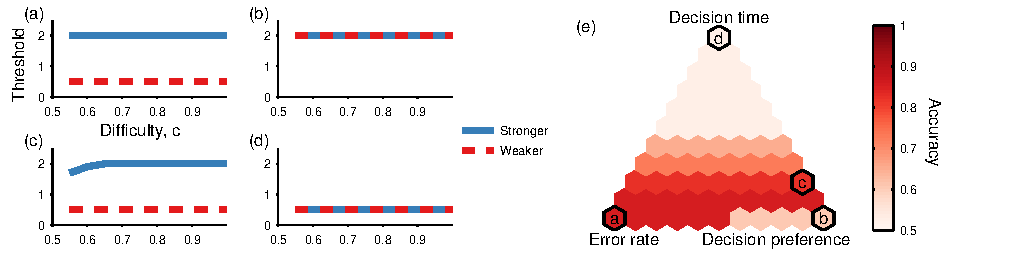
\includegraphics[width=6.83in]{Figure1.pdf}
\caption{\label{nasheq} Nash thresholds depend on the optimization weights. The accuracy of a pair using Nash equilibrium thresholds decreases as the weight given to either decision time or decision preference increases.  In (a)-(d) the lines show the Nash equilibrium thresholds for a pair of animals as a function of the difficulty of the decision ($c$). The optimization weights for each panel are indicated in the simplex with the corresponding letter. In (e) the color indicates the accuracy of a decision made by a pair making a difficult decision ($c=.55$) using Nash equilibrium thresholds, as a function of the optimization weights, $w_1$, $w_2$, $w_3$.  In the lower left corner of the simplex, only error rate matters ($w_1=1$).  In the upper corner, only decision time matters ($w_2=1$).  In the lower right corner, only preference matters ($w_3=1$). Parameters: $w_1=1$, $w_2=0$, $w_3=0$ (a), $w_1=0$, $w_2=0$, $w_3=1$ (b), $w_1=0$, $w_2=0.2$, $w_3=0.8$ (c), $w_1=0$, $w_2=0$, $w_3=1$ (d), $b=1$, $r=1$, $\ell=0.1$ in all panels. }
\end{figure*}

\begin{figure*}[ht]
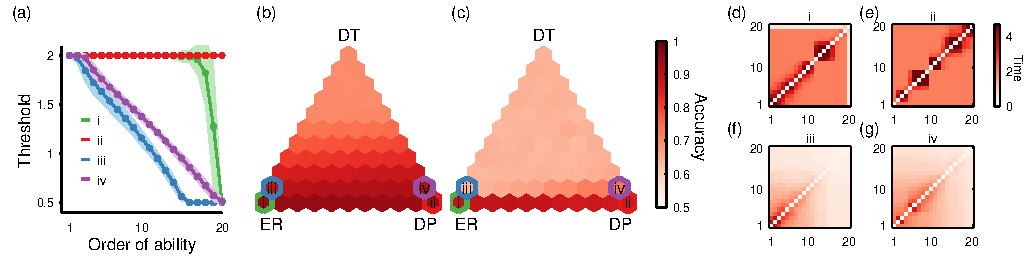
\includegraphics[width=6.83in]{Figure2.pdf}
\caption{\label{groupeq}   The accuracy of a group using Nash thresholds decreases as the weight given to decision time increases, but is not affected or increases as the weight given to decision preference increases.  In (a) the lines show the Nash thresholds as a function of position in the group for different optimization weights,  where $1$ is the strongest individual and $20$ is the weakest. The optimization weights for each panel are indicated in the simplex with the corresponding letter. The color in the simplex indicates (b) the average accuracy of the whole group and (c) the average accuracy of the decisions between individuals in the bottom quartile of a group using Nash thresholds, as a function of the optimization weights, $w_1$, $w_2$, $w_3$.  In the lower left corner of the simplex, only error rate matters ($w_1=1$).  In the upper corner, only decision time matters ($w_2=1$).  In the lower right corner, only preference matters ($w_3=1$).   In (d)-(g) the color indicates the expected time it takes each pair of components to reach a decision in a group using Nash thresholds. Parameters: $w_1=1$, $w_2=0$, $w_3=0$ (i), $w_1=0$, $w_2=0$, $w_3=1$ (ii), $w_1=0.9$, $w_2=0.1$, $w_3=0$ (iii), $w_1=0$, $w_2=0.1$, $w_3=0.9$ (iv), $N=20$, $b=1$, $r=1$, $\ell=0.1$ in all panels. }

\end{figure*}


\begin{figure}[ht]
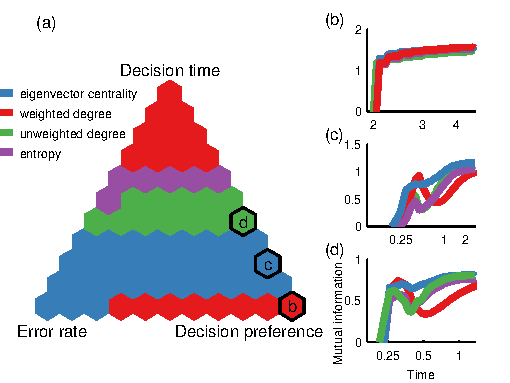
\includegraphics[width=3.4in]{Figure3.pdf}
\caption{\label{bestmetric} The best measure of consensus in the decision network depends on the average error rate and the types of errors being made.  In (a) the color indicates the most informative consensus measure to apply to a network constructed by a group using Nash thresholds, as a function of the optimization weights. In the lower left corner of the simplex, only error rate matters ($w_1=1$).  In the upper corner, only decision time matters ($w_2=1$).  In the lower right corner, only preference matters ($w_3=1$). In (b)-(d) we show how the mutual information of each consensus formalism changes over time as the network forms. The optimization weights for each panel are indicated in the simplex with the corresponding letter. Parameters: $w_1=0$, $w_2=0$, $w_3=1$ (c), $w_1=0$, $w_2=0.2$, $w_3=0.8$ (d), $w_1=0$, $w_2=0.4$, $w_3=0.6$ (e),  $N=20$, $b=1$, $r=1$, $\ell=0.1$ in all panels.}
\end{figure}


\begin{figure}[ht]
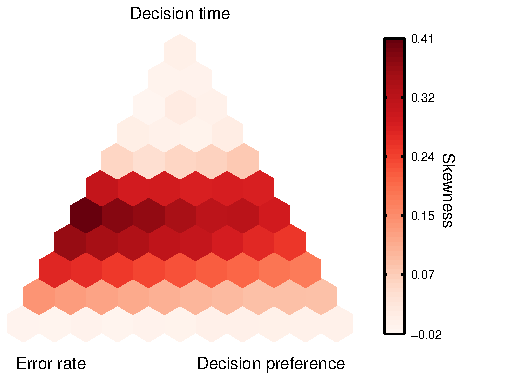
\includegraphics[width=3.4in]{Figure4}
%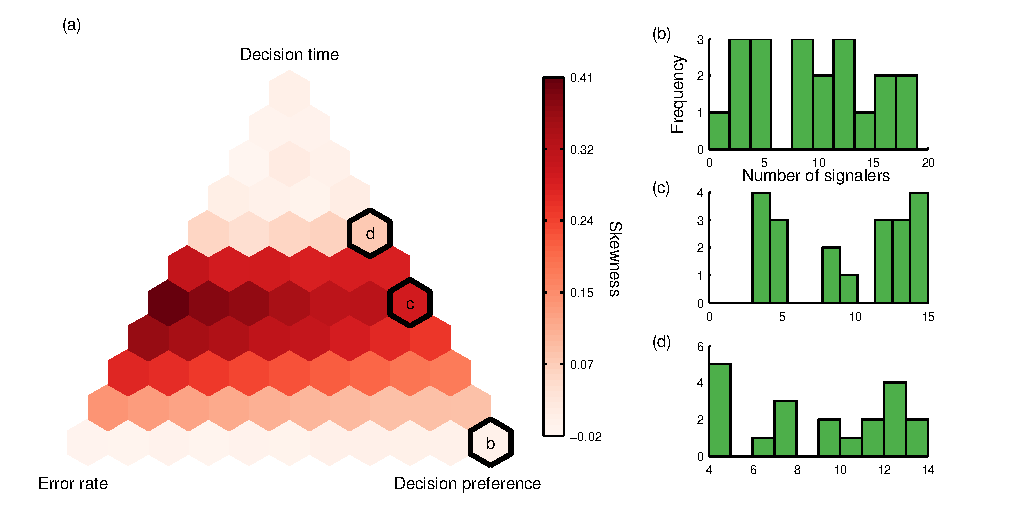
\includegraphics[width=\textwidth]{skewness_histograms.pdf}
\caption{\label{skewness} The average skewness of the distribution of unweighted in-degree is maximized at intermediate waiting costs. In the upper panel, the color indicates the average skewness of the distribution of a group using Nash thresholds, as a function of the optimization weights, $w_1$, $w_2$, $w_3$. In the lower left corner of the simplex, only error rate matters ($w_1=1$).  In the upper corner, only decision time matters ($w_2=1$).  In the lower right corner, only preference matters ($w_3=1$). Parameters: $N=20$, $b=1$, $r=1$, $\ell=0.1$.}
\end{figure}

\begin{table}[h]
\caption{\label{examples}{\bf  Examples of collective computation.} A collective computation can occur when a group of components, each of which gathers information and makes a decision in a noisy environment, produces an output that depends in a complex non-linear way on the individuals' decisions. This phenomenon is found in many biological systems. }
\begin{tabular}{@{\vrule height 10.5pt depth4pt  width0pt}llllll@{}}
System & Information & Component &   Component decision & Collective computation \\
\cline{1-5} 
brain & moving dots& neural population & to stop firing & decision of the brain
\\  social group & fights won or lost & monkey & to emit a subordination signal & power structure
\\  quorum sensing & signaling molecule & bacteria & to produce signaling molecule & production of toxin
\\ flock movement & environment & bird & where to fly and how quickly & flock movement
\\
\hline
\end{tabular}
\end{table}


\begin{table}[ht]
\caption{\label{variables}{ Variables in the model and their interpretations in neural and social systems.} }
\begin{tabular}{@{\vrule height 10.5pt depth4pt  width0pt}llllll@{}}
Variable & Definition & Neural &   Social \\
\cline{1-4} 
$a$  & value &  degree to which the property  & fighting ability
\\ & & a neural population responds to 
\\ & & is present in the environment&
\\ $b$ & change due to new evidence
\\$c$ & strength of input & coherence of dots & prob. of stronger animal winning
\\ $\ell$ & leak rate
\\ $r$ & interaction rate 
\\ $T_1,T_2$ & decision thresholds
\\ $w_1$ & error rate weight & reward from being ``right" & reward from being ``right"
\\ $w_2$ & decision time weight & penalty for taking a long time & costs of fighting
\\ $w_3$ & prob. of preference weight &  & benefit from receiving signal
\\$X_1,X_2$ & decision variables &  firing rates of neural populations & evidence accumulated about relative dominance
\\
\hline
\end{tabular}
\end{table}

\begin{table}[ht]
\centering
\caption{\label{differences}{\bf  Comparison of model in different application.} In its original application to neural systems, the leaky integrator model was reduced to one dimension and the only optimality criteria considered were accuracy and decision time. We study a two-dimensional version of the model and consider the possibility of decision preferences as an additional optimality criterion. This model can be applied to a collection of neural populations in the brain and to a social group of monkeys. Differences between the original neural application and the extended neural and social applications are highlighted in red.}
\begin{tabular}{@{\vrule height 10.5pt depth4pt  width0pt}llllll@{}}
  &Original neural & Extended neural & Social \\
\cline{1-3} \cline{4-4} 
decision & difference hits a threshold  & ? & \fcolorbox{red}{white}{one var. hits a threshold}
\\dimensionality & $1$  & $?$ & $2$  
\\ group size & $2$ &\fcolorbox{red}{white}{$N$}& \fcolorbox{red}{white}{$N$}
\\ optimality criterion &  reward from being ``right" & reward from being ``right"& reward from being ``right"
\\ & decision time &decision time & decision time
\\ & &\fcolorbox{red}{white}{reward from  receiving signal} & \fcolorbox{red}{white}{reward from  receiving signal}
\\optimization & no &  \fcolorbox{red}{white}{yes} & \fcolorbox{red}{white}{yes} 
\\ depends on other
\\  individual's threshold
\\ \hline
\end{tabular}
\end{table}




\end{document}


